\chapter{Testing}

\section{Test Plan}

\begin{landscape}
\subsection{Original Outline Plan}

\begin{center}
    \begin{tabular}{|p{2cm}|p{5cm}|p{5cm}|p{4cm}|}
        \hline
        \textbf{Test Series} & \textbf{Purpose of Test Series} & \textbf{Testing Strategy} & \textbf{Strategy Rationale}\\ \hline
        Example & Example & Example & Example \\ \hline
    \end{tabular}
\end{center}

\subsection{Changes to Outline Plan}

\begin{center}
    \begin{tabular}{|p{2cm}|p{5cm}|p{5cm}|p{4cm}|}
        \hline
        \textbf{Test Series} & \textbf{Purpose of Test Series} & \textbf{Testing Strategy} & \textbf{Strategy Rationale}\\ \hline
        Example & Example & Example & Example \\ \hline
    \end{tabular}
\end{center}

\subsection{Original Detailed Plan}

\begin{center}
    \begin{longtable}{|p{1.5cm}|p{2.5cm}|p{2.5cm}|p{2cm}|p{2cm}|p{2cm}|p{2cm}|p{2cm}|}
        \hline
        \textbf{Test Series} & \textbf{Purpose of Test} & \textbf{Test Description} & \textbf{Test Data} & \textbf{Test Data Type (Normal/ Erroneous/ Boundary)} & \textbf{Expected Result} & \textbf{Actual Result} & \textbf{Evidence}\\ \hline
       1.1 & Check new user first name input validation & Test the first name input box in the new profile window to see if it validates a name properly & Bob & normal & The name should be accepted and this will be shown by the border of the input box going green & The test worked as expected & Figure \ref{fig:test_1.1_result} on page \pageref{fig:test_1.1_result} \\ \hline
       1.2 & Check new user first name input validation & Test the first name input box to see if it tests for an invalid input properly & B0b & erroneous & The input will be rejected and this will be signified by the name box going red & Test did not go as expected - The data was accepted and the box border went green & Figure \ref{fig:test_1.2_result} on page \pageref{fig:test_1.2_result}\\ \hline
       1.3 & Check new user last name input validation & Test the last name input box to see if it tests for a valid name properly & sMiTh & normal & The input should be accepted and the box border will go green to show this & The test worked as expected & Figure \ref{fig:test_1.3_result} on page \pageref{fig:test_1.3_result}\\ \hline
       1.4 & Check the new user last name input validation & Test the last name input box to see if it tests for an invalid name properly & \$mith & erroneous & The input should be rejected and this will be shown by the border of the box going red & The test worked as expected & Figure \ref{fig:test_1.4_result} on page \pageref{fig:test_1.4_result}\\ \hline
       1.5 & Check the new user password input validation & Test the password input box to see if it tests for a valid input with normal data provided & PaSsWoRd & normal & The password should be accepted and the border for the input box will go green & the test worked as expected & Figure \ref{fig:test_1.5_result} on page \pageref{fig:test_1.5_result} \\ \hline
       1.6 & Check the new user password input validation & Test the password input box to see if it tests for a valid input with boundary data provided & PaSs & boundary & The password should be accepted and the border for the input box will go green & The test worked as expected &  Figure \ref{fig:test_1.6_result} on page \pageref{fig:test_1.6_result}\\ \hline
       1.7 & Check the new user password input validation & Test the password input box to see if it tests for an invalid input with erroneous data provided & PaS & erroneous & The password should be rejected and the border for the input will go red & The test worked as expected & Figure \ref{fig:test_1.7_result} on page \pageref{fig:test_1.7_result}\\ \hline
       1.8 & Check the new user confirm button & Test the confirm button to see if it adds data to the database & see normal data from tests above & normal & the data should be accepted and added to the database and the input window should close & the test worked as expected & Figure \ref{fig:test_1.8_result} on page \pageref{fig:test_1.8_result}\\ \hline
       2.1 & Check the `Add Reading' input window & Test the `Add Reading' window to see if it adds the required data properly & Gas, 5.276, 27th February & normal for all & The data should be added to the database & The test worked as expected & Figure \ref{fig:test_2.1_result} on page \pageref{fig:test_2.1_result}\\ \hline
       2.2 & Check the `Add Reading' input window & Test the `Add Reading' window to see if it rejects erroneous data & abcde & erroneous & the data should not be added & The test did not work as expected - erroneous data was added & Figure \ref{fig:test_2.2_result} on page \pageref{fig:test_2.2_result} \\ \hline
       2.3 & Check the `Edit Reading' input window & Test the `Edit Reading' window to see if it changes the consumption reading properly & 3.141 & normal & The data should be changed without any other data being changed & The test worked as expected & Figure \ref{fig:test_2.3_result} on page \pageref{fig:test_2.3_result}\\ \hline
       2.4 & Check the `Edit Reading' input window & Test the `Edit Reading' window to see if it changes the date properly & 28th February & normal & The date should be changed without changing any other data & The test worked as expected & Figure \ref{fig:test_2.4_result} on page \pageref{fig:test_2.4_result}\\ \hline
       2.5 & Check the `Remove Reading' input window & Test the `Remove Reading' window to see if it removes data properly & abcde & normal & The data should be removed & The test worked as expected & Figure \ref{fig:test_2.5_result} on page \pageref{fig:test_2.5_result} \\ \hline
       3.1 & Check the `Add Cost' input window & Test the `Add Cost' window to see if it adds cost data properly & Gas, 5.32, 27th February & normal & The data should be added to the database & The test worked as expected & Figure \ref{fig:test_3.1_result} on page \pageref{fig:test_3.1_result} \\ \hline
       3.2 & Check the `Add Cost' input window & Test the `Add Cost' window to see if it rejects erroneous data & qwerty & erroneous & The data should not be added &  The test didn't work as expected - data added instead of being rejected & Figure \ref{fig:test_3.2_result} on page \pageref{fig:test_3.2_result} \\ \hline
       3.3 & Check the `Edit Cost' input window & Test the `Edit Cost' window to see if it edits the consumption cost properly & 7.25 & normal & The cost consumption should be changed with other data from the same entry in the database uneffected & The test worked as expected & Figure \ref{fig:test_3.3_result} on page \pageref{fig:test_3.3_result} \\ \hline
       3.4 & Check the `Edit Cost' input window & Test the `Edit Cost' window to see if it edits the cost start date properly & 26th February & normal & The date should be changed without effecting any other data in the same entry & The test worked as expected & Figure \ref{fig:test_3.4_result} on page \pageref{fig:test_3.4_result}\\ \hline
       3.5 & Check the `Remove Cost' input window & Test the `Remove Cost' window to see if it removes a cost entry properly & qwerty & normal & The data should be removed from the database & The test worked as expected & Figure \ref{fig:test_3.5_result} on page \pageref{fig:test_3.5_result}\\ \hline
       4.1 & Check the `Add Type' input window & Test the `Add Type' window to see if it adds normal data properly & Example Type, Example Description & normal & The data should be added & The test worked as expected & Figure \ref{fig:test_4.1_result} on page \pageref{fig:test_4.1_result}\\ \hline
       4.2 & Check the `Add Type' input window & Test the `Add Type' window to see if it rejects erroneous data & F00 Description, B4r Type& erroneous & The data should be rejected and not added to the database & The test did not work as expected - data was added & Figure \ref{fig:test_4.2_result} on page \pageref{fig:test_4.2_result}\\ \hline
       4.3 & Check the `Edit Type' input window & Test the `Edit Type' window to see if it edits the type name properly & FOOBAR & normal & The type name should be changed without effecting anything else & The test didn't work as expected - Type name not changed and description completely removed & Figure \ref{fig:test_4.3_result} on page \pageref{fig:test_4.3_result}\\ \hline
       4.4 & Check the `Edit Type' input window & Test the `Edit Type' window to see if it edits the type description properly & BARFOO & normal & The type description should be changed without effecting anything else & The test worked as expected  & Figure \ref{fig:test_4.4_result} on page \pageref{fig:test_4.4_result} \\ \hline
       4.5 & Check the `Remove Type' window & Test the `Remove Type' Window to see if it removes a type entry properly & F00 Description & normal & The entry should be removed & The test worked as expected & Figure \ref{fig:test_4.5_result} on page \pageref{fig:test_4.5_result} \\ \hline
       5.1 & Check the bar chart display & Test the bar chart display & Cost, 2015-02-27 & Normal & A bar chart should be displayed showing the different consumptions for each type if available for the selected day with options to change the date and consumption type and refresh the chart & The test worked as expected & Figure \ref{fig:test_5.1_results} on page \pageref{fig:test_5.1_results} \\ \hline
       5.2 & Check the pie chart display & Test the pie chart display & Reading, 2015-02-28 & Normal & A pie chart should be displayed showing the different percentage consumptions for each type if available for the selected day with options to change the date and consumption type and refresh the chart & The test worked as expected & Figure \ref{fig:test_5.2_results} on page \pageref{fig:test_5.2_results}\\ \hline
       5.3 & Check the scatter graph display & Test the scatter graph display & Reading, 2015-02-27 & Normal & A Scatter graph should be displayed showing the different consumptions for each type if available for a selected day with options to change the date and consumption type and refresh the chart & The test did not work as expected - scatter graph not fully generated and  no options to change between the reading and cost tables & Figure \ref{fig:test_5.3_results} on page \pageref{fig:test_5.3_results}\\ \hline
       5.4 & Check the line chart display & Test the line chart display & Cost, 2015-02-27 & normal & A line graph should display for each consumption type if available showing the relevant data for the selected table and options to change the table and date and refresh the chart & The test didn't work as expected - chart not properly generated & Figure \ref{fig:test_5.4_results} on page \pageref{fig:test_5.4_results} \\ \hline
       5.5 & Check the table display & Test the table display & User & normal & A table should display showing data from the selected database table with options to change the table and if relevant, the consumption type & Works as expected & Figure \ref{fig:test_5.5_results} on page \pageref{fig:test_5.5_results}\\ \hline
    \end{longtable}
\end{center}

\subsection{Changes to Detailed Plan}

\begin{center}
    \begin{longtable}{|p{1.5cm}|p{2.5cm}|p{2.5cm}|p{2cm}|p{2cm}|p{2cm}|p{2cm}|p{2cm}|}
        \hline
        \textbf{Test Series} & \textbf{Purpose of Test} & \textbf{Test Description} & \textbf{Test Data} & \textbf{Test Data Type (Normal/ Erroneous/ Boundary)} & \textbf{Expected Result} & \textbf{Actual Result} & \textbf{Evidence}\\ \hline
        Example & Example & Example & Example & Example & Example & Example & Example \\ \hline
    \end{longtable}
\end{center}
\end{landscape}
\section{Test Data}

\subsection{Original Test Data}

\begin{center}
\begin{tabular}{|p{1.5cm}|p{2cm}|p{2cm}|}
	\hline
	\textbf{Test Series} & \textbf{Test Data}& \textbf{Test Data Type} \\ \hline
	1.1 & Bob & normal \\ \hline
	1.2 & B0b & erroneous\\ \hline
	1.3 & sMiTh & normal\\ \hline
	1.4 & \$mith & erroneous\\ \hline
	1.5 & PaSsWoRd & normal \\ \hline
	1.6 & PaSs & boundary \\ \hline
	1.7 & PaS & erroneous \\ \hline
	2.1 & Gas & normal \\ \hline
	2.1 & 5.276 & normal \\ \hline
	2.1 & 27th february & normal \\ \hline
	2.2 & abcde & erroneous \\ \hline
	2.3 & 3.141 & normal \\ \hline
	2.4 & 28th February & normal \\ \hline
	2.5 & abcde & normal \\ \hline
	3.1 & gas, 5.32, 27th february & normal \\ \hline
	3.2 & qwerty & erroneous \\ \hline
	3.3 & 7.25 & normal \\ \hline
	3.4 & 26th february & normal \\ \hline
	3.5 & qwerty & normal \\ \hline
	4.1 & Example Type, Example Description & normal \\ \hline
	4.2 & F00 Description, B4r Type & erroneous \\ \hline
	4.3 & FOOBAR & normal \\ \hline
	4.4 & BARFOO & normal \\ \hline
	4.5 & F00 Description & normal \\ \hline
	5.1 & Cost, 2015-02-27 & Normal \\ \hline
	5.2 & Reading, 2015-02-28 & Normal \\ \hline
	5.3 & Reading, 2015-02-27 & Normal \\  \hline
	5.4 & Cost, 2015-02-27 & Normal \\ \hline
	5.5 & User & Normal \\ \hline
\end{tabular}
\end{center}
	
\subsection{Changes to Test Data}

\section{Annotated Samples}

\subsection{Actual Results}

\subsection{Evidence}
\begin{figure}[H]
	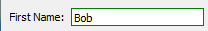
\includegraphics{./testing/images/test_1_1_first_name_input_normal.png}
	\caption{The result of testing the first name input for adding a new user with normal data} \label{fig:test_1.1_result}
\end{figure}
	
\begin{figure}[H]
	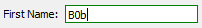
\includegraphics{./testing/images/test_1_2_first_name_input_erroneous.png}
	\caption{The result of testing the first name input for adding a new user with erroneous data} \label{fig:test_1.2_result}
\end{figure}

\begin{figure}[H]
	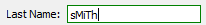
\includegraphics{./testing/images/test_1_3_last_name_input_normal.png} 
	\caption{The result of testing the last name input for adding a new user with normal data} \label{fig:test_1.3_result}
\end{figure}

\begin{figure}[H]
	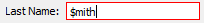
\includegraphics{./testing/images/test_1_4_last_name_input_erroneous.png}
	\caption{The result of testing the last name input for adding a new user with erroneous data} \label{fig:test_1.4_result}
\end{figure}

\begin{figure}[H]
	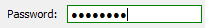
\includegraphics{./testing/images/test_1_5_password_input_normal.png}
	\caption{The result of testing the password input for adding a new user with normal data} \label{fig:test_1.5_result}
\end{figure}

\begin{figure}[H]
	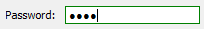
\includegraphics{./testing/images/test_1_6_password_input_boundary.png}
	\caption{The result of testing the password input for adding a new user with boundary data} \label{fig:test_1.6_result}
\end{figure}

\begin{figure}[H]
	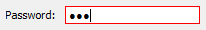
\includegraphics{./testing/images/test_1_7_password_input_erroneous.png}
	\caption{The result of testing the password input for adding a new user with erroneous data} \label{fig:test_1.7_result}
\end{figure}

\begin{figure}[H]
	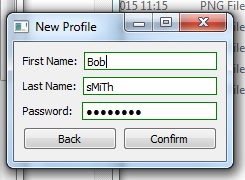
\includegraphics{./testing/images/test_1_8_confirm_button_data.png}
	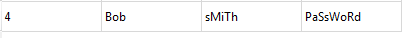
\includegraphics{./testing/images/test_1_8_confirm_button_data_added.png}
	\caption{The result of testing the confirm button for adding a new user with normal data} \label{fig:test_1.8_result}
\end{figure}

\begin{figure}[H] 
	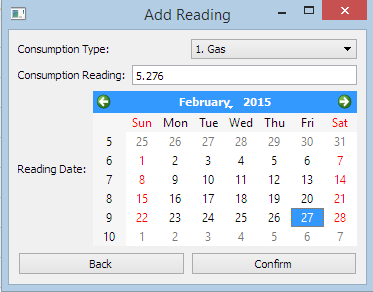
\includegraphics{./testing/images/test_2_1_add_reading_data.png}
	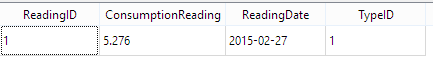
\includegraphics{./testing/images/test_2_1_add_reading_data_added.png}
	\caption{The result of testing the `add reading' window with normal data} \label{fig:test_2.1_result}
\end{figure}

\begin{figure}[H]
	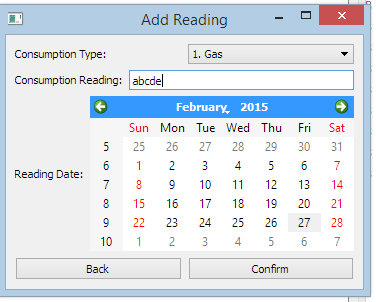
\includegraphics{./testing/images/test_2_2_add_reading_data_erroneous.png}
	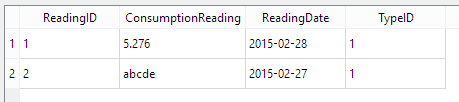
\includegraphics{./testing/images/test_2_2_add_reading_data_erroneous_added.png}
	\caption{The result of testing the `add reading' window with erroneous data} \label{fig:test_2.2_result}
\end{figure}

\begin{figure}[H]
	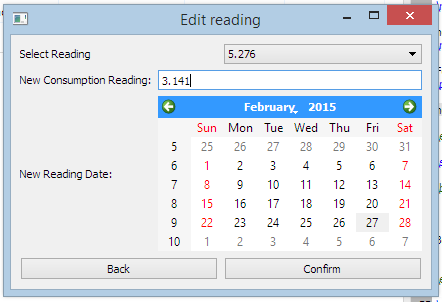
\includegraphics{./testing/images/test_2_3_edit_reading_consumption_data.png}
	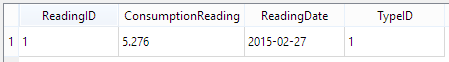
\includegraphics{./testing/images/test_2_3_edit_reading_consumption_before.png}
	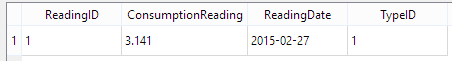
\includegraphics{./testing/images/test_2_3_edit_reading_consumption_data_changed.png}
	\caption{before and after edit consumption date} \label{fig:test_2.3_result}
\end{figure}

\begin{figure}[H]
	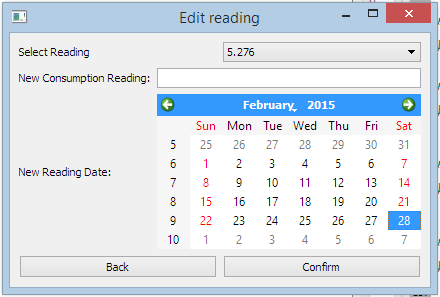
\includegraphics{./testing/images/test_2_4_edit_reading_date_data.png}
	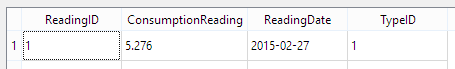
\includegraphics{./testing/images/test_2_4_edit_reading_date_before.png}
	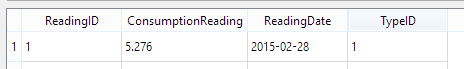
\includegraphics{./testing/images/test_2_4_edit_reading_date_data_changed.png}
	\caption{before and after edit consumption date} \label{fig:test_2.4_result}
\end{figure}

\begin{figure}[H]
	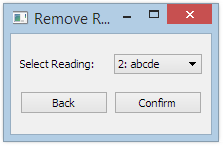
\includegraphics{./testing/images/test_2_5_remove_reading_data.png}
	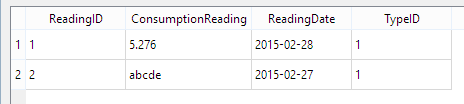
\includegraphics{./testing/images/test_2_5_remove_reading_before.png}
	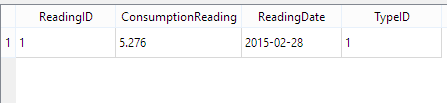
\includegraphics{./testing/images/test_2_5_remove_reading_removed.png}
	\caption{before and after remove reading} \label{fig:test_2.5_result}
\end{figure}

\begin{figure}[H]
	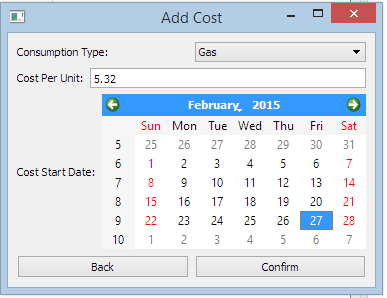
\includegraphics{./testing/images/test_3_1_add_cost_data.png}
	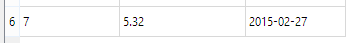
\includegraphics{./testing/images/test_3_1_add_cost_added.png}
	\caption{The result of testing the `add cost' window with normal data} \label{fig:test_3.1_result}
\end{figure}

\begin{figure}[H]
	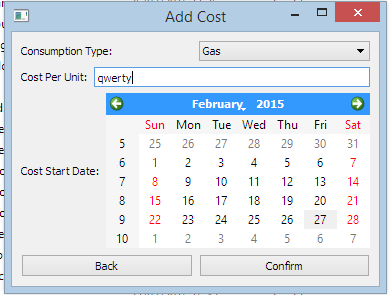
\includegraphics{./testing/images/test_3_2_add_cost_erroneous_data.png}
	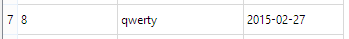
\includegraphics{./testing/images/test_3_2_add_cost_erroneous_added.png}
	\caption{The result of testing the `add cost' window with erroneous data} \label{fig:test_3.2_result}
\end{figure}

\begin{figure}[H]
	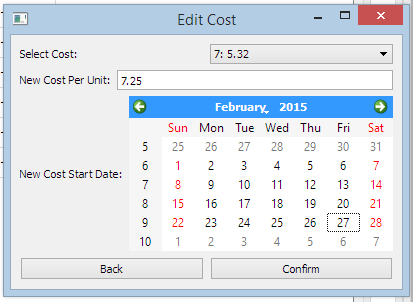
\includegraphics{./testing/images/test_3_3_edit_cost_price_data.png}
	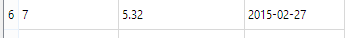
\includegraphics{./testing/images/test_3_3_edit_cost_price_before.png}
	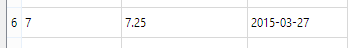
\includegraphics{./testing/images/test_3_3_edit_cost_price_after.png}
	\caption{Before and After edit cost consumption price} \label{fig:test_3.3_result}
\end{figure}

\begin{figure}[H]
	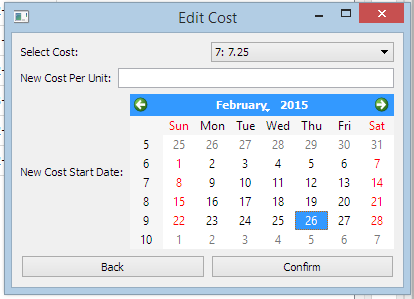
\includegraphics{./testing/images/test_3_4_edit_cost_date_data.png}
	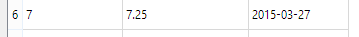
\includegraphics{./testing/images/test_3_4_edit_cost_date_before.png}
	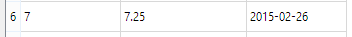
\includegraphics{./testing/images/test_3_4_edit_cost_date_after.png}
	\caption{Before and After edit cost consumption date} \label{fig:test_3.4_result}
\end{figure}

\begin{figure}[H]
	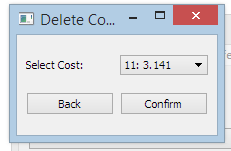
\includegraphics{./testing/images/test_3_5_remove_cost_data.png}
	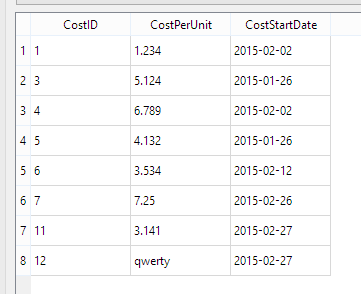
\includegraphics{./testing/images/test_3_5_remove_cost_before.png}
	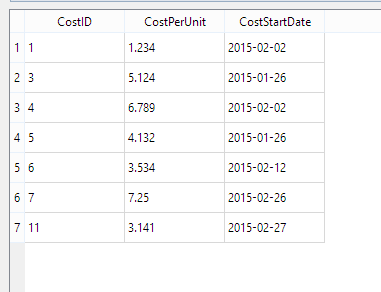
\includegraphics{./testing/images/test_3_5_remove_cost_after.png}
	\caption{Before and After remove cost entry} \label{fig:test_3.5_result}
\end{figure}

\begin{figure}[H]
	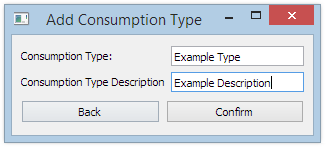
\includegraphics{./testing/images/test_4_1_add_type_data.png}
	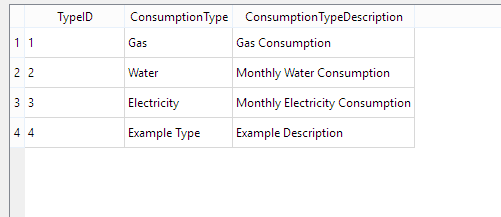
\includegraphics{./testing/images/test_4_1_add_type_added.png}
	\caption{The result of testing the `Add Type' window with normal data} \label{fig:test_4.1_result}
\end{figure}

\begin{figure}[H]
	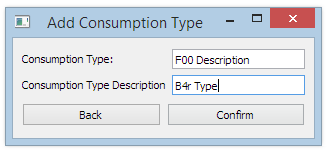
\includegraphics{./testing/images/test_4_2_add_type_data_erroneous.png}
	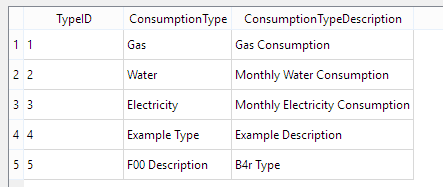
\includegraphics{./testing/images/test_4_2_add_type_erroneous_added.png}
	\caption{The result of testing the `Add Type' window with erroneous data} \label{fig:test_4.2_result}
\end{figure}

\begin{figure}[H]
	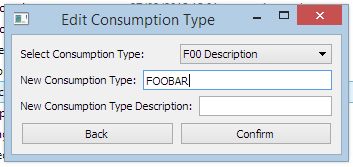
\includegraphics{./testing/images/test_4_3_edit_type_name_data.png}
	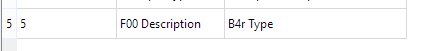
\includegraphics{./testing/images/test_4_3_edit_type_name_before.png}
	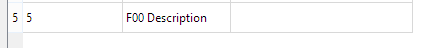
\includegraphics{./testing/images/test_4_3_edit_type_name_after.png}
	\caption{Before and After of editing the consumption type name} \label{fig:test_4.3_result}
\end{figure}

\begin{figure}[H]
	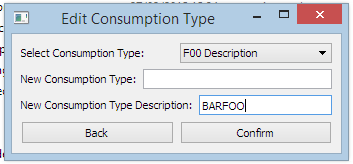
\includegraphics{./testing/images/test_4_4_edit_type_description_data.png}
	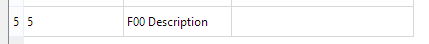
\includegraphics{./testing/images/test_4_4_edit_type_description_before.png}
	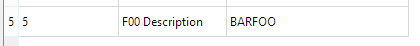
\includegraphics{./testing/images/test_4_4_edit_type_description_after.png}
	\caption{Before and After editing the consumption type description} \label{fig:test_4.4_result}
\end{figure}

\begin{figure}[H]
	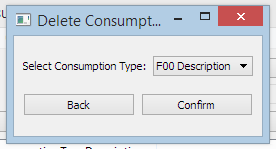
\includegraphics{./testing/images/test_4_5_remove_type_data.png}
	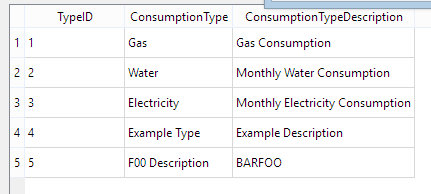
\includegraphics{./testing/images/test_4_5_remove_type_before.png}
	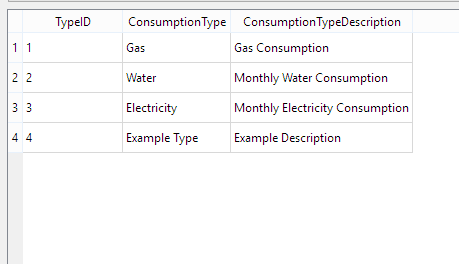
\includegraphics{./testing/images/test_4_5_remove_type_after.png}
	\caption{Before and After removing a type entry} \label{fig:test_4.5_result}
\end{figure}

\begin{figure}[H]
	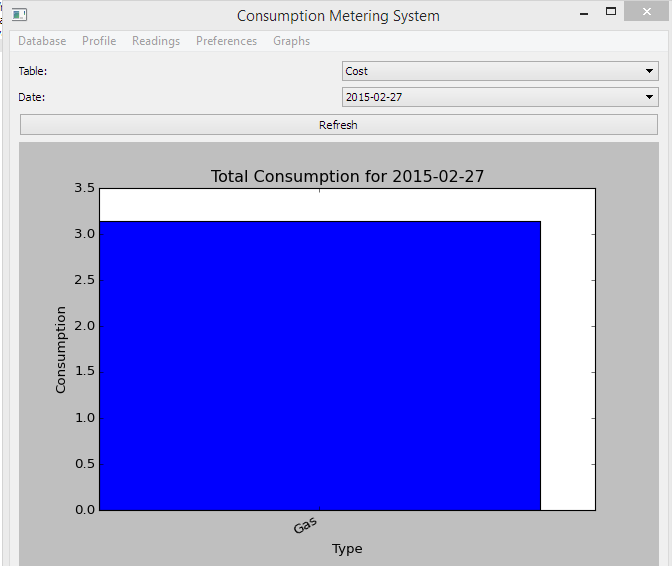
\includegraphics{./testing/images/test_5_1_barchart.png}
	\caption{Bar chart test} \label{fig:test_5.1_results}
\end{figure}

\begin{figure}[H]
	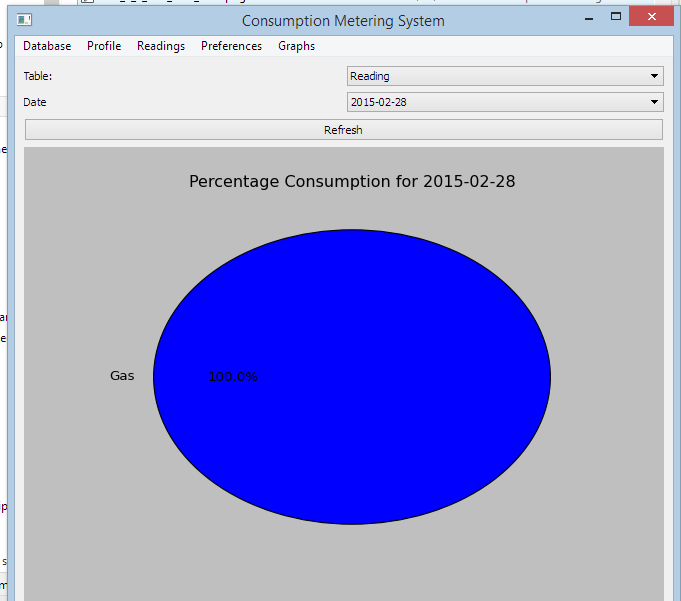
\includegraphics{./testing/images/test_5_2_piechart.png}
	\caption{Pie chart test} \label{fig:test_5.2_results}
\end{figure}

\begin{figure}[H]
	\includegraphics{./testing/images/test_5_3_scattergraph.png}
	\caption{Scatter graph test} \label{fig:test_5.3_results}
\end{figure}

\begin{figure}[H]
	\includegraphics{./testing/images/test_5_4_linegraph.png}
	\caption{Line graph test} \label{fig:test_5.4_results}
\end{figure}

\begin{figure}[H]
	\includegraphics{./testing/images/test_5_5_table.png}
	\caption{Table test} \label{fig:test_5.5_results}
\end{figure}

\section{Evaluation}

\subsection{Approach to Testing}
To test my system I created, I took a linear approach in which I went through the menu bar and tested each option individually with normal, boundary and erroneous data where relevant. The reason I used this method is because it is easy to do and makes it easier to tell which parts I've tested and which parts I have not tested

\subsection{Problems Encountered}
In the testing I found a few problems with my system such as:
\begin{itemize}
	\item The validation of the first name and last name - accepts special characters when it shouldn't. See Figure \ref{fig:test_1.2_results} on page \pageref{fig:test_1.2_results}
	\item The system doesn't reject erroneous data from the add reading window. See Figure \ref{fig:test_2.2_results} on page \pageref{fig:test_2.2_results}
	\item The system doesn't reject erroneous data from the add cost window. See Figure \ref{fig:test_3.2_results} on page \pageref{fig:test_3.2_results}
	\item The system doesn't reject erroneous data from the add type window. See Figure \ref{fig:test_4.2_results} on page \pageref{fig:test_4.2_results}
	\item The system doesn't edit the consumption type data properly - when just attempting to edit the consumption type name it doesn't get changed and the consumption type description gets removed. See Figure \ref{fig:test_4.3_results} on page \pageref{fig:test_4.3_results}
	\item The system doesn't display the scatter graph layout properly - scatter graph doesn't generate and no option to select the database table. See Figure \ref{fig:test_5.3_results} on page \pageref{fig:test_5.3_results}
	\item The system doesn't display the line graph layout properly - line graph doesn't generate. See Figure \ref{fig:test_5.4_results} on page \pageref{fig:test_5.4_results}
\end{itemize}

\subsection{Strengths of Testing}
The strengths of my testing approach are:
\begin{itemize}
	\item It is easy to do
	\item It is easy to know which parts have been tested
	\item It is easy to know which parts have not been tested
\end{itemize}
	
\subsection{Weaknesses of Testing}
\begin{itemize}
	\item It is slow to do
	\item It can get tedious
\end{itemize}

\subsection{Reliability of Application}

\subsection{Robustness of Application}